% Final Tex File for
% Econometrics 2 Problem Set 4

% PLEASE INSERT YOUR NAME IN LINE 87
% If you want a different title appearance, comment out line 109!

\documentclass[%
  fontsize=11pt, % Schriftgröße
  version=last,%  % Neueste Version von KOMA-Skript verwenden
  headsepline,
  titlepage = false,
  DIV = 11, % Größe Textfeld
  abstract = false
]{scrartcl}

% penalties
\clubpenalty = 100000
\widowpenalty = 100000

% packages
\usepackage[utf8]{inputenc}
\usepackage[english]{babel} % 'british' ergibt andere Datumsformate als 'english'

%------------------------------------------------------------------------------------------------

% text and page appearances
\usepackage{textcomp}
\usepackage{verbatim}
\usepackage{comment}
\usepackage{setspace}
\usepackage{geometry} %Seitenränder
%\geometry{top=25mm, left=30mm, right=30mm, bottom=25mm,
%headsep=10mm, footskip=12mm}
\usepackage{scrlayer-scrpage}
\usepackage{pdfpages}

%\usepackage[official]{eurosym} % Euro Sign

% math packages
\usepackage{mathtools}
\usepackage{amssymb}
\usepackage{amsmath}
\usepackage{amsthm}
%\numberwithin{equation}{section} % to count equations by chapter and section
%\usepackage{siunitx}
%\usepackage{xfrac}

% lists
\usepackage{mdwlist}
\usepackage{paralist}
\usepackage{enumitem}

% references
\usepackage{varioref}
\usepackage{hyperref}
\usepackage{cleveref}

% images, tables in floating environments
\usepackage{float}
\usepackage{subfig}
\usepackage[section]{placeins} % float fence at each section (figure and table environment)
%\usepackage[percent]{overpic} % put titles & descriptions in latex on pictures through a grid positioning
\usepackage{booktabs}
\usepackage{tabularx}
%\numberwithin{figure}{section} % to count figures by section
%\numberwithin{table}{section}
\usepackage{rotating} % rotate figure/table environments
\usepackage{lscape}

% FONTS-------------------------------------------------------------------------------------------

\usepackage{lmodern} % updated standard latex font
%\setkomafont{title}{\bfseries \rmfamily} % special font for title section, perhaps dropping the sans serif?
%\setkomafont{section}{\bfseries \Large \rmfamily} % same as above for section titles
%\setkomafont{pageheadfoot}{\large \rmfamily} % size of head/foot font, also type of font

% temporary packages to solve problems
%\usepackage[round]{natbib} % align with Karo
\renewcommand{\thesubsection}{\alph{subsection}} % count subsections using the alphabet (alternative to enumeration here!)
%\usepackage{dcolumn} % to make the stargazer tables work

% KOMA SCRIPT-------------------------------------------------------------------------------------

% info variables for komascript  Generate Title, Author & Date in Headline
\makeatletter
\title{Metrics 2 Assignment 4} % TITEL
\author{Vorname Nachname}	% NAME
\pagestyle{scrheadings}
% Put Title, Author & Date in Headline
%\titlehead{\today} % redundant in most cases, but if you need date in different title setups, put it in here
\ihead{\@author} % heading, inner part of page (left in default case unless scrbook)
\ohead{\today} % heading, outer part
\chead{\@title} % heading, always in center

% COMMANDS------------------------------------------------------------------------------------------

% proprietary commands
\onehalfspacing
%\renewcommand{\theenumi}{\textbf{\alph{enumi}}} % enumerations use lower-case letters instead of numbers on 1st level. relevant for exercise 2
%\graphicspath{{   }}   % Insert path to directory for plot files (maybe the cd from stata?)

% my commands
\newcommand{\meth}{Methamphetamine} % i just cannot spell this word... and neither decide whether to put it upper or lower-case

%%%%%%%%%%%%%%%%%%%%%%%%%%%%%%%%%%%%%%%%%%%%%%%%%%%%%%%%%%%%%%%%%%%%%%%%%%%%%%%%%%%%%%%%%%%%%%%%%%

\begin{document}
% Alternative Title No 1
\maketitle % dropping this command just prints the headpiece on page 1 as well

% Alternative Title No 2
%\begin{center}
%{\Huge \textbf{\@title} }
%\bigskip 
%\bigskip 
%{\large \@author}\\
%\bigskip 
%{\large \today}\\
%\end{center}

\section*{Exercise 1: DiD - Paper discussion}
\subsection*{Research Question}
The authors' main goal is to assess the effectiveness of enforcement efforts aimed at reducing the consumption of \meth~ in the US. More specifically, they want to size up the impact of state restrictions on three aspects: Firstly the sales of retail cold medicines used to produce \meth~ on the production; secondly, the consumption of it and thirdly drug related arrests.\\
The authors investigate the effects on both the supply and the demand side. Since it is the (legislation's) ultimate goal to reduce drug consumption, we believe that the focus should be shifted rather towards the consumers. The investigation on the consumer side is restricted on one type of drugs. Thereby, the analysis fails to acknowledge consumers' substitution towards similar drugs (e.g. ecstasy). On top of that, it would be interesting to shed more light on the interaction between effects on the supply and the demand side.

\subsection*{Contribution}
It is proclaimed that the paper contributes to the literature by offering more credible estimates by analysing the success of a smaller, but more typical enforcement effort. This accounts for the problem that evaluating large enforcement efforts might no be a good predictor of the effects induced by typical enforcement efforts. Thus, analysing smaller enforcement efforts yields higher external validity. The authors claim that the combination of specific regulation and its well-defined and known implementation as well as rich administrative data sets is essential for the contribution of this paper.\\
It is clear that so far there exists no consensus in the literature regarding the effectiveness of enforcement efforts in reducing drug use. Thus, the paper contributes to the existing literature by providing empirical evidence from a different angle.

\subsection*{Aim of the Analyzed Policy}
%Reduction of diversion of ephidrine and pseudoephridine to reduce availability of methamphetime. Specifically, controls on OTC cold and sinus medications.
The aim of the analyzed policy is the reduction of \meth use by addressing the channel of drug production. In particular, the policy consists of the following measures:
\begin{itemize*}
	\item Sales limits and product placement
	\item Implementation of purchasing quotas, Placement in secure areas (35 states)
	\item Inspection of ID
	\item Implementation of logbook (24 states)
\end{itemize*}

\subsection*{Meth(odology)}
The method of Difference-in-differences (DiD) is applied in order to reliably identify causal effects by ruling out endogeneity of regressors. The causal effect is measured relative to a control group which has not received the treatment yet. This helps to control for factors that are correlated with the treatment dummy as well as the error term. Time and state fixed effects further capture omitted variables. 
\\ Event studies constitute an important tool checking for non-linear trends relative to the implementation of the law. Adding linear state-specific time trends and further controls is useful to evaluate whether the identification assumptions for DiD are fulfilled.\\
There is no control group, hence the classical DiD design is not feasible here. This is not good for validity. One might suspect some form of endogeneity since states facing larger problems with \meth~ consumption are expected to implement the legislation rather sooner than later. Hence, the treatment is not randomly assigned between states. Furthermore, the design does not account for heterogeneity across states regarding the total production of \meth. They only deliver an ATE but not a LATE or MTE conditional on the pre-treatment Meth production, which might be more insightful.\\


\subsection*{Identifying Variation}
The identifying variation is the variation in the timing of states' implementation of the OTC regulations. Without this variation, the time fixed effects would absorb the event-time dummies entirely making identification impossible. 

\subsection*{Key Identifying Assumption}
The Key Identifying Assumption in DiD models in general is the common trend assumption. As they control for state specific linear and quadratic time trends, the key identifying assumption only requires that there are no unmeasured non-linear and non-quadratic state specific trends correlated with the enactment of the regulations. This is hard to test and seems plausible by the authors' explanation.

\subsection*{Data}
Administrative data from various sources:
\begin{itemize}
	\item Data for \meth production:
	\begin{itemize*}
		\item NCLSS: Seized/Discovered labs
		\item STRIDE: purity and price of methamphetamine
	\end{itemize*}
	\item Data for \meth consumption:
	\begin{itemize*}
		\item HCUP: positive drug tests (workers) \\ \textit{Only from Jan 2000 - Apr 2006}
		\item HCUP (NIS - Nationwide Inpatient Samples): positive drug tests (hospital admissions) \\ \textit{From Jan 2000 - Dec 2007}
	\end{itemize*}
	\item Data on drug-related arrests
	\begin{itemize*}
		\item UCR: arrests for posession and sale of illegal drugs \\ \textit{From Jan 2000 - Dec 2007; Reporting voluntar}y
	\end{itemize*}
\end{itemize}

Without naming any reasons, the dataset is restricted to the time period from 2000 to 2007. The dataset is not very homogeneous over the time dimension as it is a combination from various sources. Furthermore, it is lacking information on how many drug stores / pharmacies actually comply with the new regulation (and in return does not reveal the number of never-takers). After all, Missouri enacted similar restrictions already in 2003 but this is not included in the dataset. %Now our trust is shattered and who knows what else is wrong?

\subsection*{Results/Findings}
Aim of the policy is achieved judging by figures 2 \& 3. The suppliers of \meth seem to have taken a hit. \\
\meth~ production
\begin{itemize}[noitemsep, topsep=1pt]
	\item Production capacity:
	The estimation results suggest that the laws caused a 36$\%$ reduction in the number of methamphetamine laboratories, with the largest decline among labs with capacity between 2-8 oz (54\%). Furthermore, it hints that the enforcement efforts lead to a decline of 25$\%$ in the domestic production of methamphetamine.
	\item Purity and price:
	There is a large drop in purity in 2005, but also changes in purity before the enactment of the law. There is no change in the nominal price.
\end{itemize} \vspace{0.5em}
\meth~consumption
\begin{itemize}[noitemsep, topsep=1pt]
	\item No significant impact of regulations on drug test outcomes for workers and inpatients.
\end{itemize} \vspace{0.5em}
Drug related arrests
\begin{itemize}[noitemsep, topsep=1pt]
	\item There is no evidence that restrictions reduced drug related arrests. 
\end{itemize} \vspace{0.5em}
Spatial spillovers
\begin{itemize}[noitemsep, topsep=1pt]
	\item Evidence that there exist spillover effects reducing the regulation's impact on production when the neighbouring state did not implement the law. When the neighbouring state implements the law, this effect vanishes and the reduction of \meth~production converges to the level of non-border counties.
\end{itemize}
Regression table 1 shows that the coefficient of interest does not change considerably over the different specifications. The high robustness of the results supports the identification assumption. 

\subsection*{Interpretation of the Results/Implications/Policy Relevance}
The implications of the paper are twofold: On the one hand, enforcement efforts do significantly reduce the supply of \meth, on the other hand, they do not have an impact on the market equilibrium regarding price and quality, suggesting that there are no effects on consumption. To draw policy conclusions, as mentioned earlier, it would be crucial to understand why the observed reduction in the supply of \meth~is not reflected in a decrease in consumption. It would be necessary to shed more light on the interaction between effects on the supply and the demand side. Further, when drawing implications for policy makers, some limitations of the paper should be considered (see next point).

\subsection*{Limitations of the Paper}
One clear shortcoming is the fact that the paper only analyzes data for the discovered labs. The findings are based on the assumption that the probability of the lab being seized remains constant after the introduction of the law. Thereby, incentives of the police to lower investigation efforts are not considered. Furthermore, it is imaginable that that there is a development towards more professional producers being able to better hide their activities. \\
Moreover, the general problem might not be solved as producers substitute to other drugs that they offer to their costumers. Presumably, the policy would be more effective if it would be introduced to a broad set of different drugs. \\
There are further limitations regarding the consumer side results. The rate of consumers with positive test results is not necessarily linearly dependent of aggregated consumption. A consumer for example can reduce his consumption by one half but still has a positive test result. Noticeably, it is difficult to detect whether consumers have switched to other drugs since common tests can not reliably distinguish between different drugs. Furthermore, substitution to other drugs or changes in the amount consumed can lead to the same observed prices and purity measures although \meth~ production has decreased. \\
Moreover, the policy implications do not apply to all kinds drugs. Some drugs are mainly produced outside the US. \\
Finally, the results on drug use might be driven by self selection in the measurement of \meth~consumption: It is likely that only those patients and workers with a record of drug use will be subject to \meth~tests. 
\newpage

\section*{Exercise 2: DiD - practical application}



% Enable line 74 to use the \subsection command counting with letters as an alternative below
\subsection{} % a)
	\begin{figure}[H]
		\centering
		\caption{Replication of Figure 2 of Dobnik et al. (2014)}		\label{fig:Fig2}
		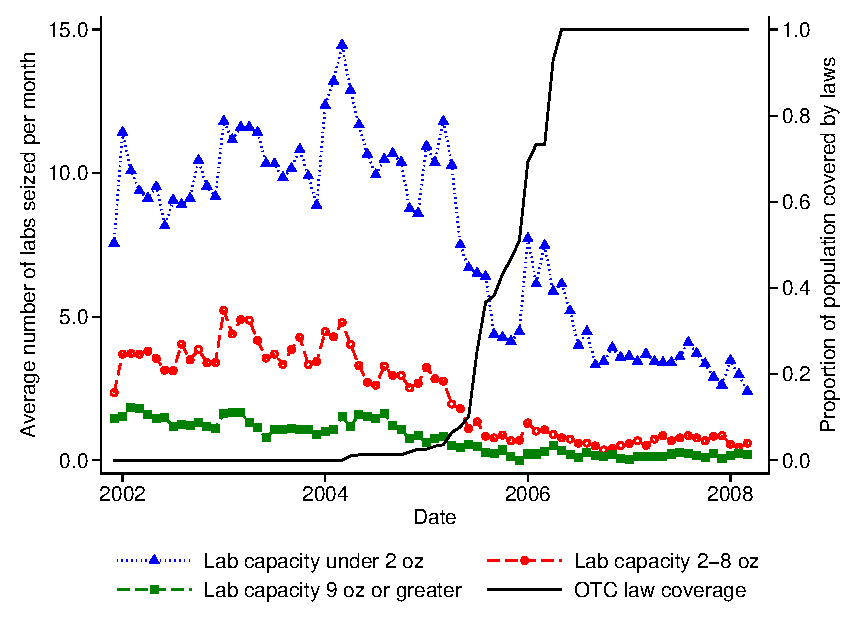
\includegraphics[width=0.85\textwidth]{Figure2_Replication.eps}
	\end{figure}
Figure 1 reveals a clearly negative relationship between the number of labs seized per month and the proportion of population covered by the law. The decrease in the average number of labs seized per month is the largest the smaller the lab capacity (in absolute terms). The plot suggests that the introduction of the law was effective in reducing the average number of labs seized. However, further regression analysis is necessary in order to identify causal links. \\
\newpage
%
\subsection{} % b)
	\begin{figure}[H]
	\centering
	\caption{Average number of labs discovered in event time by lab size} 	\label{fig:Figb}
	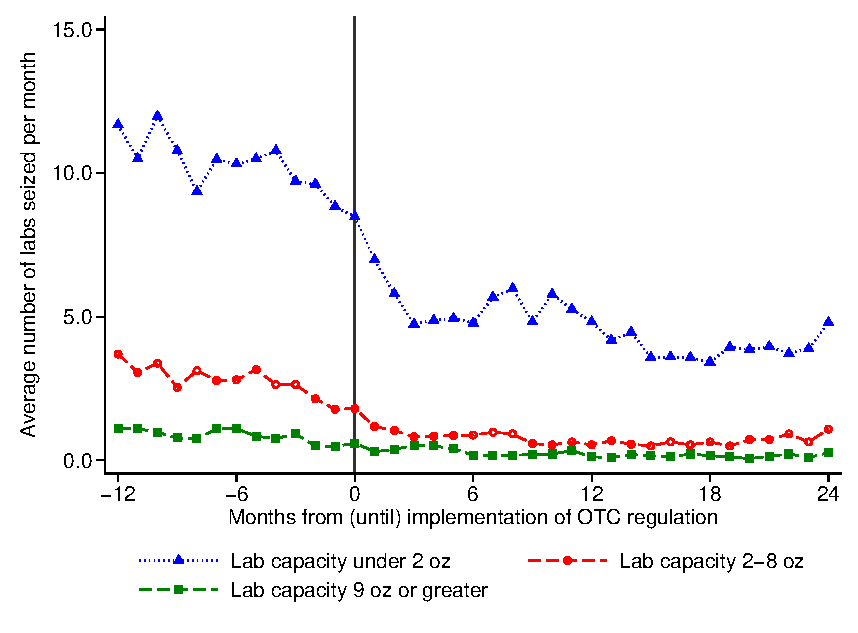
\includegraphics[width=0.85\textwidth]{Figure_Exercise_b.eps}
%	\begin{minipage}{0.95\textwidth}
%		{\footnotesize \textit{Sources:}  \newline
%		\textit{Notes:} \par}
%	\end{minipage}
\end{figure}


%
\subsection{} % c)
\begin{center}
\begin{tabular}{lcccc} \hline
 & (1) & (2) & (3) & (4) \\
 & Small labs & Medium labs & Large labs & All labs \\
VARIABLES & cap\_under\_2\_oz & cap\_2\_8\_oz & cap\_9\_oz & tot\_labs \\ \hline
 &  &  &  &  \\
OTC & -4.059*** & -2.141*** & -0.276 & -6.477*** \\
 & (1.171) & (0.513) & (0.315) & (1.821) \\
 &  &  &  &  \\
Observations & 4,937 & 4,937 & 4,937 & 4,937 \\
R-squared & 0.142 & 0.195 & 0.075 & 0.186 \\
 Number of states & 50 & 50 & 50 & 50 \\ \hline
\multicolumn{5}{l}{ Robust standard errors in parentheses} \\
\multicolumn{5}{l}{ *** p$<$0.01, ** p$<$0.05, * p$<$0.1} \\
 &  &  &  &  \\
\end{tabular}
\end{center}
\newpage
To calculate the standard errors, we cluster on the state level because it is likely that the timing of the treatment depends on the state (for example due to institutional patterns).  \\
The estimated coefficients are close to the ones found in the paper (see Regression Table 1, specification 1). They slightly differ because we include the whole time sample and further do not have data for Florida. The results coincide with what we see on the plots: There is a negative effect of the law on the number of labs seized which is the more negative the smaller the lab size. The DiD regression results indicate a persistent effect which is also depicted by the graphs. Otherwise the coefficients would not be significantly different from zero.
%
\subsection{} % d)

\begin{itemize}
	\item DiD common trend assumption: Consistency of the estimated regression requires that there are no state specific 		trends that are correlated with the OTC variable. Common trends are covered by the time fixed effects. Regression Table 1 reveals that the inclusion of a state specific linear and quadratic trend leads to estimates slightly closer to zero. Given that the coefficients do not change considerably, we expect the assumption to hold more or less. To detect whether the inclusion changes the coefficient one would need to perform a Wald test. 
	
	\item Fixed effects assumption: Consistency of the estimated regression requires that state and time fixed effects are not correlated with the error term.
	
	\item DiD assumption no effect prior to the treatment (DiD.3): This assumption is questionable since some states implemented the law at a later point in time than other states which presumably implies anticipation effects.
	
	\item DiD.1,DiD.2 and DiD.5 hold.
\end{itemize}

\subsection{} % e)
Equation 1 restricts the treatment effect to be constant over time. Beta estimates the average treatment effect across time and state. Equation 2 allows for variation of the treatment effect over time but still not across states. This is more flexible and provides interesting insights into the temporary evolution.
\newpage

\subsection{} % f)
\begin{figure}[th]
	\centering
	\caption{Estimates of event time dummies}	\label{fig:Figf}
	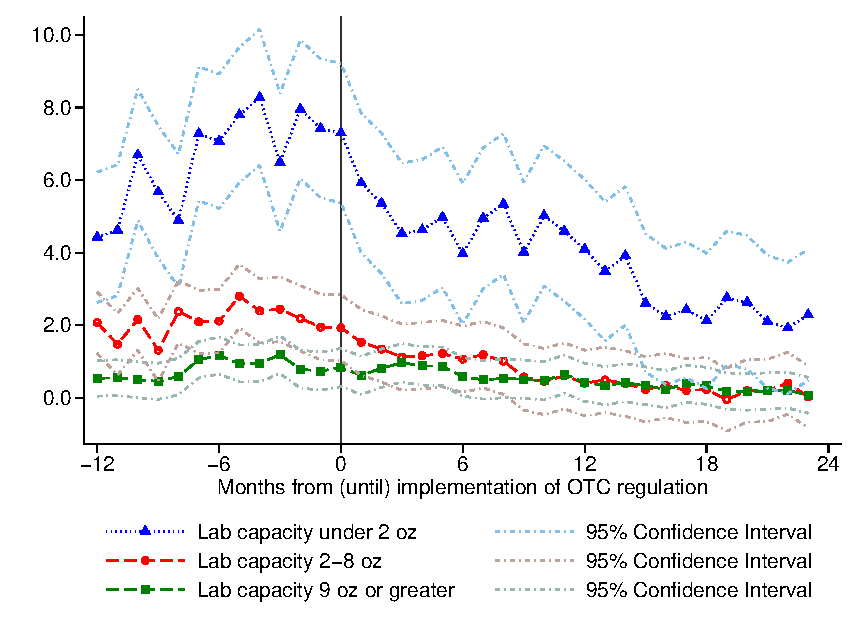
\includegraphics[width=0.85\textwidth]{Figure_exercise_f.eps}
%	\begin{minipage}{0.95\textwidth}
%		{\footnotesize \textit{Sources:}  \newline
%		\textit{Notes:} \par}
%	\end{minipage}
\end{figure}

The dynamics look similar to the previous findings. The number of small labs reduces considerably over time. The effect is not so clear regarding mid-size and large labs. The effect looks quite persistent.


%%% THE END %%%
\end{document}

